\documentclass{beamer}

\usepackage{graphicx}
\usepackage{caption}
\usepackage{subcaption} % for subfigure
\usepackage{hyperref}
\usepackage{amssymb}
\usepackage{tabularx}
\usepackage{multicol}
\usepackage{algpseudocode}
\usepackage{amsthm} % for theorem
\usepackage{algorithm}
\usetheme{Warsaw}
\title[Inter-procedural \& Concurrent HRA] % (optional, only for long titles)
{Inter-Procedural Heap Reference Analysis for Concurrent Programs}
\subtitle{BTP Presentation}
\author[Anshul Purohit] % (optional, for multiple authors)
{
Anshul Purohit \\
Roll No: 110050002 \\
}
\institute[Universitäten Hier und Dort] % (optional)
{
	
}
\date[KPT 2004] % (optional)
{
Guide: Prof. Uday Khedkar \\
}
\subject{Informatik}


\begin{document}
\frame{\titlepage}
\begin{frame}

\frametitle{Outline}
\begin{itemize}
\item Introduction to Problem Statement
\item Heap Analysis 
\item Inter-Procedural Analysis
\item Analysis of Concurrent Programs
\item Design of analysis and tools
\end{itemize}
\end{frame}

  \begin{frame}
    \frametitle{Introduction - Flow Sensitivity}
    \tableofcontents[Introduction to Problem Statement]

Data flow analysis is a technique for gathering program information at various points in a program. The value is then propagated in the Control Flow graph (CFG) of the program. It can be classified in two types:

\begin{itemize}
	\item  Flow-insensitive analysis ignores the control-flow graph, and assumes that statements can execute in any order.
	\item Flow-sensitive analysis takes control flow structure of program into account.	
\end{itemize}
  \end{frame}
  
  \begin{frame}
    \frametitle{Introduction - Interprocedural Analysis}

\begin{itemize}
	
	\item Inter-procedural analysis extends the scope of data flow analysis across procedure boundaries.
	\item It incorporates the effects of procedure calls in the caller procedures and calling contexts in the callee procedure.
	\item A context-sensitive analysis is an \textbf{inter-procedural analysis} which reanalyzes callee procedure for each context. \item Context insensitive analysis performs analysis independent of calling context.
	
\end{itemize}
	\end{frame}
	
	
  \begin{frame}
  \frametitle{Introduction - Problem Statement}
  \begin{itemize}
  \item Designing a framework for carrying
  out inter-procedural analysis of concurrent programs and then implement heap reference analysis using the framework.
  \item Determining the information like liveness,
  accessibility and points-to information of reference expressions.
  \item Reference expression like \emph{x.lptr.rptr.data} are primarily used to access the objects in the heap.
  \item Java model: The root variables, which are stored on stack, represent references to memory in heap.
     
  \end{itemize}
  \end{frame}
  
  \begin{frame}
  	\frametitle{Introduction - Concurrency}
  	
  	 Model of threads used to refer to concurrent programs in the problem.
  	\begin{itemize}
  		\item Need to define a run method. Invoking the run method starts concurrent thread execution.
  		\item For accessing shared data,
  		critical sections need to be guarded by the lock and unlock statements.
  		\item High level abstractions of concurrency can be modeled in terms of threads. Thread library handles spawning, joining and synchronization of threads. 
  		
  	\end{itemize}
  	
  \end{frame}
  
  \begin{frame}
\frametitle{Heap Analysis}
	Analyzing properties of heap data is not very trivial.  

\begin{itemize}
	\item The structure of stack and static data is simple to understand. 
	\item Stack variables have a compile-time name(alias) associated with it.
	\item However, heap data has no compile time alias associated. Also the mapping of access expressions to memory location can change during program execution.
	\item Objects are referred based on their allocation site.
\end{itemize}
  \end{frame}
  
  
  
  
% RELATED WORK %
  \begin{frame}
  \frametitle{Heap Analysis}
  %\framesubtitle{Related Work}
	Heap analysis tries to find out the answer to the questions: 
	\begin{itemize}
		\item Can an access expression $a_1$ at program point $p_1$ have the same l-value as access expression $a_2$ at program  point $p_2$.
		\item Can there exist objects in the heap that will not be reachable from the access expressions in the program?
		\item Which of the access links will be live at a particular point?
	\end{itemize}
	\end{frame}
\begin{frame}
\frametitle{Points-to analysis for Java}
  %\framesubtitle{Related Work}
	In Java pointers are not created explicitly. All objects in Java are accessed using references. Points-to analysis for Java programs identifies the objects pointed to by references at run time.
	
	\begin{figure}[here]
	\begin{center}
	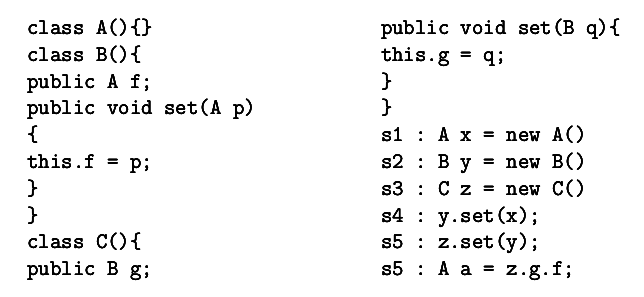
\includegraphics[width=8cm]{Figures/rsz_heap.png}
	\end{center}
	\caption{Example for heap access and points-to}
	\label{fig:ex1}
	\end{figure}
	
	
	
  \end{frame}

  \begin{frame}
  \frametitle{Points-to Graph}
  %\framesubtitle{Related Work}
	Points-to graph in Java contain two types of edges. The first type of edge is to represent the information that reference variable $v$  is pointing to object $o$. The second type of edge represents the field $f$ of $o_1$ pointing to $o_2$.

	\begin{figure}[here]
		\begin{center}
			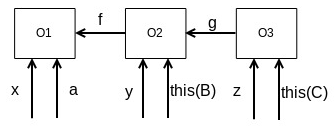
\includegraphics[width=7cm]{Figures/rsz_points_to_graph.png}
		\end{center}
		\caption{Example for points-to graph}
		\label{fig:ex1}
	\end{figure}

  \end{frame}

\begin{frame}
\frametitle{Heap Reference Analysis}

A reference can be represented by an access path. In order to perform liveness analysis of heap and identify the set of live links, naming of links is necessary.

%An Access Path is defined as root variable name following any number of field names and is represented as $x$ $\rightarrow$ $n_1$ $\rightarrow$ $n_2$ .... $\rightarrow$ $n_k$ where $x$ is root variable, $n_1$ , $n_2$ .. $n_k$ are field names.

	\begin{figure}[here]
		\begin{center}
			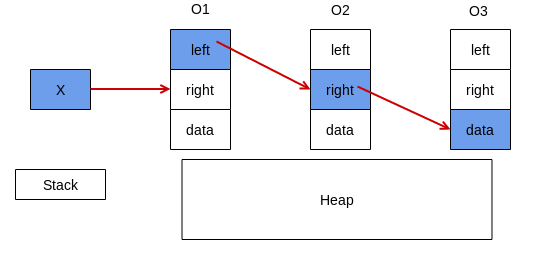
\includegraphics[width=8cm]{Figures/hra_access_path.png}
		\end{center}
		\caption{access path for the expression \emph{x.left.right.data}}
		\label{fig:accpath}
	\end{figure}

\end{frame}

\begin{frame}
\frametitle{Heap Liveness Analysis}

An access path can be unbounded in the case of loops. We need to set a bound on the representation of access paths for liveness information. This is achieved using access graphs. Summarization would also require including program points.

\begin{figure}[here]
	\begin{center}
		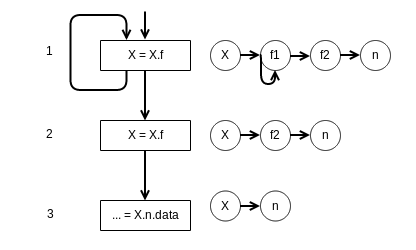
\includegraphics[width=7cm]{Figures/heap_summarization_liveness.png}
	\end{center}
	\caption{Use of access graph and liveness data flow values}
	\label{fig:accpath}
\end{figure}

\end{frame}

\begin{frame}
\frametitle{Availability and Anticipability}
	\begin{itemize}
		\item An access path $\rho$ is said to available at a program point $p$ if the target of each prefix of $\rho$ is guaranteed to be created along each path reaching $p$.
		\item An access path $\rho$ is said to be anticipable at $p$ if the target of each prefix of $\rho$ will be dereferenced along every path starting from $p$.
		\item Access graphs are not needed to carry out available and anticipable analysis over heap data because the sets are bounded. This is due to the nature of the problem (over all paths).
	\end{itemize}
\end{frame}

% RULE SETS %
  \begin{frame}
  \frametitle{Inter-procedural analysis}
  %\framesubtitle{Analysing existing rule sets}
  Inter-procedural Analysis is required to obtain more precise results as it is very common that programs can have multiple function calls.
  \begin{itemize}
	\item It is essential to consider the effect of function call on the data flow value entering the node.
	\item Inter-procedural analysis takes into account call return , parameter passing , local variables of the function, return values and recursion into account
	\item Major issue to be dealt while handling inter-procedural analysis is to deal with calling contexts.
	\end{itemize}
  \end{frame}
  
  \begin{frame}
  \frametitle{Context Sensitivity}
  %\framesubtitle{Analysing existing rule sets}
\begin{itemize}
	\item Context insensitive analysis over-approximates inter-procedural control flow. Invalid return control paths are accessed.
	\item Context sensitive analysis takes into account the calling context, thus only valid return paths are considered.
	\item Context sensitivity plays an important role in Java as it is an OO language. Data access is indirect through method calls.
\end{itemize}

  \end{frame}
  
  \begin{frame}
  \frametitle{Call Graph}
  %\framesubtitle{Analysing existing rule sets}
  \begin{itemize}
  	\item Static data structure representing run-time calling relationships among procedures.
  	\item Call multi-graph is a directed graph which represents calling relationships.
  	\item In Super graph callsites are connected to the callee procedure entry node and the exit node is connected to return node in the caller.
  \end{itemize}

  \end{frame}

  \begin{frame}
  \frametitle{Example}
  		\begin{figure}[here]
  			\begin{center}
  				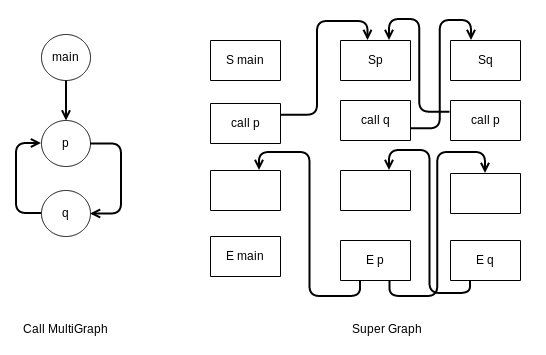
\includegraphics[width=10cm]{Figures/callgraph.png}
  			\end{center}
  			\caption{Call Multi-graph and super graph examples}
  			\label{fig:cmg_sg}
  		\end{figure}
  \end{frame}
  
  \begin{frame}
  \frametitle{Approaches to Inter-procedural Analysis.}
  \framesubtitle{Functional}
  \begin{itemize}
  	\item Summary flow functions are computed for each function. 
  	\item Directly apply the summarized flow function for handling call. Summarized flow function is dependent on the callee.
  	\item Iterative computation of summary flow function would be need till fixed point is achieved. Guaranteed to terminate only for finite lattices. 
  \end{itemize}	

  \end{frame}

  \begin{frame}
  \frametitle{Approaches to Inter-procedural Analysis.}
  \framesubtitle{Call Strings}
   %\vspace{\baselineskip}
  Call string at a program point is the sequence of unfinished calls reaching that point starting from the main procedure call.\vspace{\baselineskip}
  
  The data flow equations are changed to incorporate the merging of the data flow values only if the contexts(call strings) are the same.\vspace{\baselineskip}
  
  At a call node $c_i$ , $c_i$ is appended to the call-string value at that point. Similarly at a return node the last call site ci is removed. For recursive programs, number of call strings can be infinite. \vspace{\baselineskip}
  
  Value termination of Call Strings : Grouping into equivalence classes if they have same data flow value at the start node.
  \end{frame}
  
  \begin{frame}
  \frametitle{Approaches to Inter-procedural Analysis.}
  \framesubtitle{Value Context Method}
  Combination of the two views of contexts: data flow values at call site are stored as value contexts and call strings as calling contexts. 
  \vspace{\baselineskip}
  
  A value context is defined by a particular data flow value reaching a procedure. It is used to enumerate and tabulate the summary flow function of the procedure in terms of input and output data flow values.  

  \vspace{\baselineskip}
  When a new call to a procedure is encountered, the value context table is consulted to decide if the procedure needs to be analyzed again.
  
  
  \end{frame}
  
  \begin{frame}
  \frametitle{Approaches to Inter-procedural Analysis.}
  \framesubtitle{Value Context Method}
	 A calling context transition table is maintained  allowing flow of information along inter-procedurally valid paths. 
	
	\vspace{\baselineskip}
	Transitions are recorded in the form ( ($X$,$c$) , $Y$) where $X$ represents calling context, $c$ represents call site and $Y$ represents callee context.
	
	\vspace{\baselineskip}
	 
	
  \end{frame}
  
  \begin{frame}
  	\frametitle{Example of value context method}
  	\begin{figure}[here]
  		\begin{center}
  			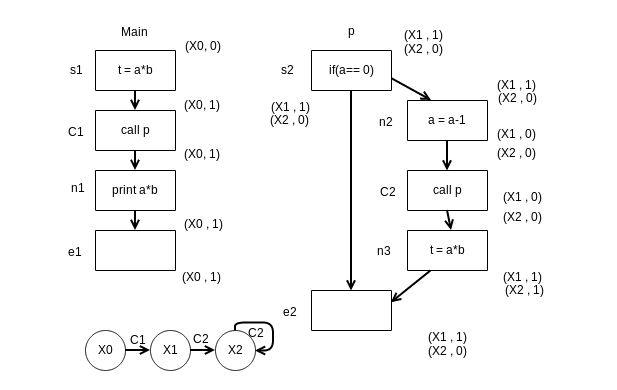
\includegraphics[width=7cm]{Figures/avbl_exp_interproc.png}
  		\end{center}
  		\caption{Example for inter-procedural available analysis}
  		\label{fig:extreme}
  	\end{figure}
  \end{frame}
  
  \begin{frame}
  \frametitle{Example of value context method}
\begin{figure}[here]
\begin{center}
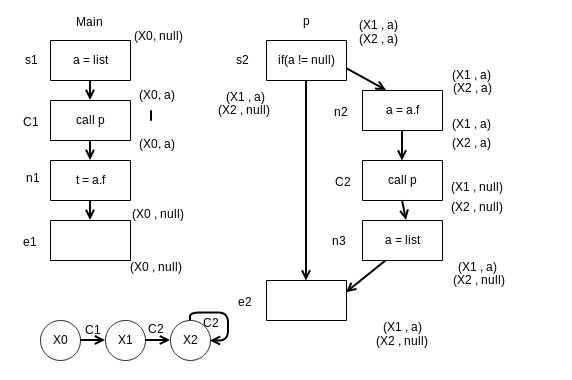
\includegraphics[width=7cm]{Figures/interproc_example.png}
\end{center}
\caption{Example for inter-procedural heap liveness}
\label{fig:extreme}
\end{figure}
	
	In the example the 2 contexts $X_1$ and $X_2$ are stored for the recursive procedure $p$.Value based contexts are used as a cache table for distinct call sites apart from terminating analysis of recursive procedures.
	
	

  \end{frame}
  
  \begin{frame}
  \frametitle{Analysis for concurrent programs}
  
  \begin{itemize}
  	\item Using the technique mentioned in the paper Dataflow Analysis for Datarace-Free Programs.
  	\item Produces an analysis for concurrent programs, given a sequential data-flow analysis
  	\item Criteria to apply this : Data flow facts should be dependent on the contents of the memory access path. This can be applied to constant propagation, not-null, liveness analysis. The program should be free of data races. 
  \end{itemize}
  
  \end{frame}
  
\begin{frame}
\frametitle{Analysis for concurrent programs}
Main challenge $\rightarrow$ converting the analysis for sequential programs to concurrent programs. How to propagate data-flow values to handle all possible thread execution order? .

\vspace{\baselineskip}
Synchronization structure of the program is made use of to propagate data-flow values

\vspace{\baselineskip}
The insight is that data-flow values are only propagated between threads at the lock and unlock points in threads. The relevant statements would usually be present inside the critical section.

\end{frame}  
  
  \begin{frame}
  \frametitle{Memory Model}
	\begin{itemize}
		\item Specifies the interactions of threads with memory and its shared use.
		\item Constraints on data access  
		\item Conditions of how data written by one thread is accessible to other threads
	\end{itemize}
	%Based on happens before-relation between two events. 
	Happens-Before Order: Statement  a happens before statement b if one of the following hold
	\begin{itemize}
		\item a appears before b in the program order
		\item b synchronizes-with a
		\item b can be reached transitively using happens-before relation from a.
	\end{itemize} 

  \end{frame}
  
\begin{frame}
\frametitle{Memory Model}

\begin{figure}
	\centering
	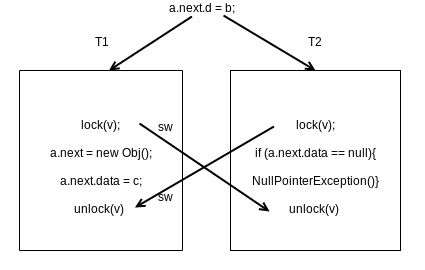
\includegraphics[width=0.6\textwidth]{Figures/sync_threads.png}
	\caption{Happens Before memory model with thread synchronization}
	\label{fig:happensbefore1}
	
	The \emph{NullPointerException} in $T_2$ cannot be raised because of the synchronizes-with relation between the lock and unlock statement. 
	
\end{figure}

\end{frame}

\begin{frame}
\frametitle{Memory Model}
\begin{figure}[b]
	\centering
	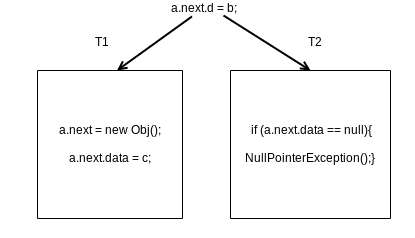
\includegraphics[width=0.5\textwidth]{Figures/sync_no_lock.png}
	\caption{Happens Before memory model without thread synchronization}
	\label{fig:happensbefore2}
\end{figure}

 	There is no synchronization relation between any statement across $T_1$ and $T_2$. There is no happens before order defined for statements across $T_1$ and $T_2$. So, NullPointerException() can be raised.
	
\end{frame}

\begin{frame}
\frametitle{Concurrent Null-Pointer Analysis}
	\begin{figure}
	\centering
	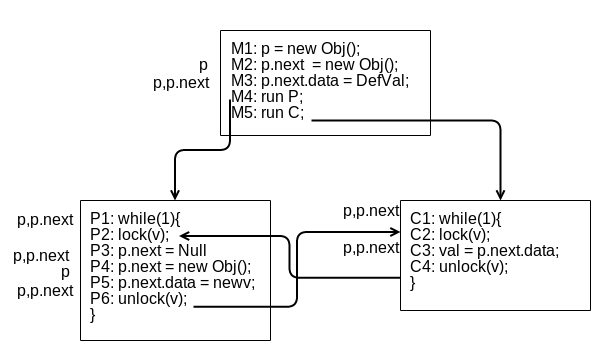
\includegraphics[width=0.75\textwidth]{Figures/concurrent_analysis.png}
	\caption{Heap Access path based null pointer analysis}
	\label{fig:nullpointeranalysis}
	\end{figure}
	
	\begin{itemize}
		\item Construction of sync-cfg by adding synchronization edges.
		\item Approximation of concurrent analysis to sequential analysis. Imprecise data flow values are obtained only at irrelevant statements.
	\end{itemize}
	 	
\end{frame}

\begin{frame}
\frametitle{Concurrent Null-Pointer Analysis}
	\begin{figure}
		\centering
		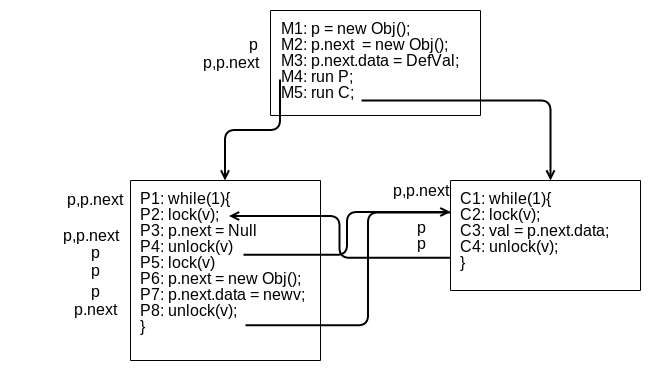
\includegraphics[width=0.75\textwidth]{Figures/concurrent_analysis_2.png}
		\caption{Heap Access path based null pointer analysis}
		\label{fig:nullpointeranalysis}
	\end{figure}
	
	Only $p$ is not-null at the statement C3, because of merging of values from P4 and P8.
	
\end{frame}

\begin{frame}
	\frametitle{Concurrent Heap Liveness Analysis}
	\begin{figure}
		\centering
		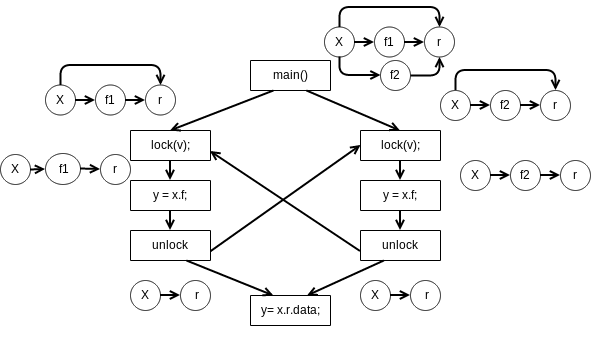
\includegraphics[width=0.7\textwidth]{Figures/concurrent_analysis_3.png}
		\caption{Concurrent Heap Liveness Analysis }
		\label{fig:nullpointeranalysis}
	\end{figure}
	Notice how the data flow value is precise only for statements within the lock-unlock section.
\end{frame}
	 
	
\begin{frame}
	\frametitle{Analysis to be Implemented}
	\begin{itemize}
		\item To implement concurrent heap liveness analysis.
		\item To extend the concurrent analysis technique to inter-procedural level using the method of value contexts. Support function calls in the critical section of the program.
	\end{itemize}
	
	
\end{frame}

\begin{frame}
	\frametitle{Sync-cfg for Concurrent Heap Liveness}
	\begin{figure}
		\centering
		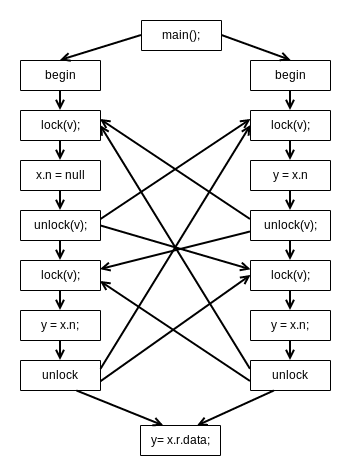
\includegraphics[width=0.5\textwidth]{Figures/hra_live_concurrent.png}
		\caption{Concurrent Heap liveness analysis input}
		\label{fig:nullpointeranalysis}
	\end{figure}
	
\end{frame}

\begin{frame}
	\frametitle{Tools to Use}
	\begin{itemize}
		\item \emph{SOOT}: Java Byte Code Optimization Framework. Can implement precise intra-procedural analysis. SPARK engine provided call graph.
		\item \emph{VASCO}: Framework for carrying out precise inter-procedural analysis. Returns a better call graph as compared to SPARK.
		\item \emph{CombinedUnitGraph}: Generation of sync-cfg for programs containing upto 2 threads. Need to extend it to $n$ threads.
	\end{itemize}
\end{frame}

\begin{frame}

\Huge Thank You

\end{frame}
\end{document}